% ju 05-Mar-24 mein-dokument.tex
\documentclass{vorlage-design-main}
\usepackage[utf8]{inputenc}
\usepackage{longtable}
\usepackage{blindtext,alltt}

%% Ganze Überschrift
\title{Anwendung von Markdown-Techniken für Dokumentationen}

%% Kürzerer Titel zur Verwendung im Seitenkopf
\runningtitle{Dokumentation mit Markdown}
\author{Jan Unger}
% \author{2.}
\date{\today}

%% Die .bib-Datei mit vollständigen Referenzen zur Verwendung mit biblatex. articleclass lädt das Paket biblatex-chicago mit Anpassungen
\addbibresource{literatur.bib}

\begin{document}

\maketitle

\begin{abstract}
In der heutigen schnelllebigen Zeit ist die Fähigkeit, komplexe
Informationen klar und effizient zu kommunizieren, von entscheidender
Bedeutung. Markdown, eine leichtgewichtige Markup-Sprache, hat sich als
ein wertvolles Werkzeug für die Erstellung technischer Dokumentationen
und die Unterstützung von Entwicklungsprojekten etabliert.

Ein weiterer Vorteil von Markdown ist die nahtlose Konvertierung in
andere Formate wie HTML und PDF durch Werkzeuge wie Pandoc, was die
Verbreitung von Dokumenten über verschiedene Plattformen und Medien
hinweg vereinfacht.
\end{abstract}

\section{Dokumente in Markdown
erstellen}\label{dokumente-in-markdown-erstellen}

\begin{lstlisting}
// Projektübersicht
Entwicklung               git_hilfsprogramm.py      mein-dokument.fls
LICENSE                   html                      mein-dokument.tex
Makefile                  image_resizer.py          navigation.css
NAVIGATION.html           images                    python-scripte
README.md                 literatur-kfz.bib         scriptauswahl.py
TODO.md                   literatur-sport.bib       tex
Tabellen                  literatur.bib             vorlage-design-main.cls
content                   md
dokumentation.py
\end{lstlisting}

Git

\begin{lstlisting}[language=bash]
# Git Versionierung
gh auth login
git config --global credential.helper cache

git remote -v

git init --bare
git remote add local /Users/jan/notizen_latex_html_python_v1.git
git remote rename localBackup local
git push local main
git pull local main

git init
git remote set-url origin https://github.com/ju1-eu/notizen_latex_html_python_v1.git
git push -u origin main
git pull origin main

git push
git pull
git  st
git ls

git clone https://github.com/ju1-eu/notizen_latex_html_python_v1.git
git clone /Users/jan/notizen_latex_html_python_v1.git notizen_klon
\end{lstlisting}

Beispiel Quellenangabe

\begin{itemize}

\item
  Fachbuchautor \textcite{dalwigk:2024:fachbuchautor}.
\item
  Online Kurse \textcite{schaffranek:2024:kurse}.
\item
  Hacking und Cyber Security mit KI \textcite{dalwigk:2023:hacking}.
\item
  Python für Einsteiger \textcite{dalwigk:2022:python}.
\item
  Mikrocontroller ESP32 \textcite{brandes:2023:mikrocontroller}.
\item
  Roboterauto \textcite{brandes:2022:esp32}.
\item
  Daten mit Raspberry Pi im Netz speichern und visualisieren
  \textcite{brandes:2023:daten}.
\end{itemize}

Hier ist ein Text, der eine Fußnote benötigt.\footnote{Text der Fußnote.}

Liste

\begin{enumerate}
\def\labelenumi{\arabic{enumi}.}

\item
  eins
\item
  zwei
\end{enumerate}

\textbf{Tabelle 1:} Diese Tabelle gibt eine übersichtliche Darstellung
der ausgeführten Skripte, ihrer jeweiligen Funktionen und der Ergebnisse
der Ausführung.

\begin{table}[ht]
  %\caption{}
  %\label{tab:my-table}
  \begin{tabular}{@{}lll@{}}
\toprule
Skriptname
 & 
Beschreibung
 & 
Ergebnis
 \\
\midrule[\heavyrulewidth]
\verb|html\_konverter\_pandoc1.py| & Konvertiert
HTML-Dokumente mit Pandoc & Erfolgreich abgeschlossen \\
\verb|html\_dateien\_verarbeiten2.py| & Verarbeitet
HTML-Dateien & Erfolgreich abgeschlossen \\
\verb|navigationsseite\_html.py| & Erzeugt
Navigationsseiten mit Jinja2 & Fehler: Modul `jinja2' nicht gefunden \\
\verb|html\_entfernen2.py| & Bearbeitet die Datei
mein-dokument.html & Erfolgreich abgeschlossen \\
\bottomrule
\end{tabular}%
\end{table}

\newpage

\begin{lstlisting}[language={C++}]
// Quellcode: HalloWelt.cpp
#include <iostream>

int main() {
    std::cout << "Hallo Welt" << std::endl;
    return 0;
}
\end{lstlisting}

\begin{lstlisting}
// Markdown
[Google](https://www.google.com)

![Logo 2](images/Logo/Logo2.pdf)
\end{lstlisting}

Website \href{https://www.google.com}{Google} und GitHub
\url{https://github.com/ju1-eu} und meine Website
\url{https://bw-ju.de/}

\begin{figure}
\centering

\includegraphics[width=0.8\textwidth]{images/Logo/Logo2.pdf}
%\floatnotes{}
%\label{fig:}
\caption{Logo 2}
\end{figure}

\begin{figure}
\centering
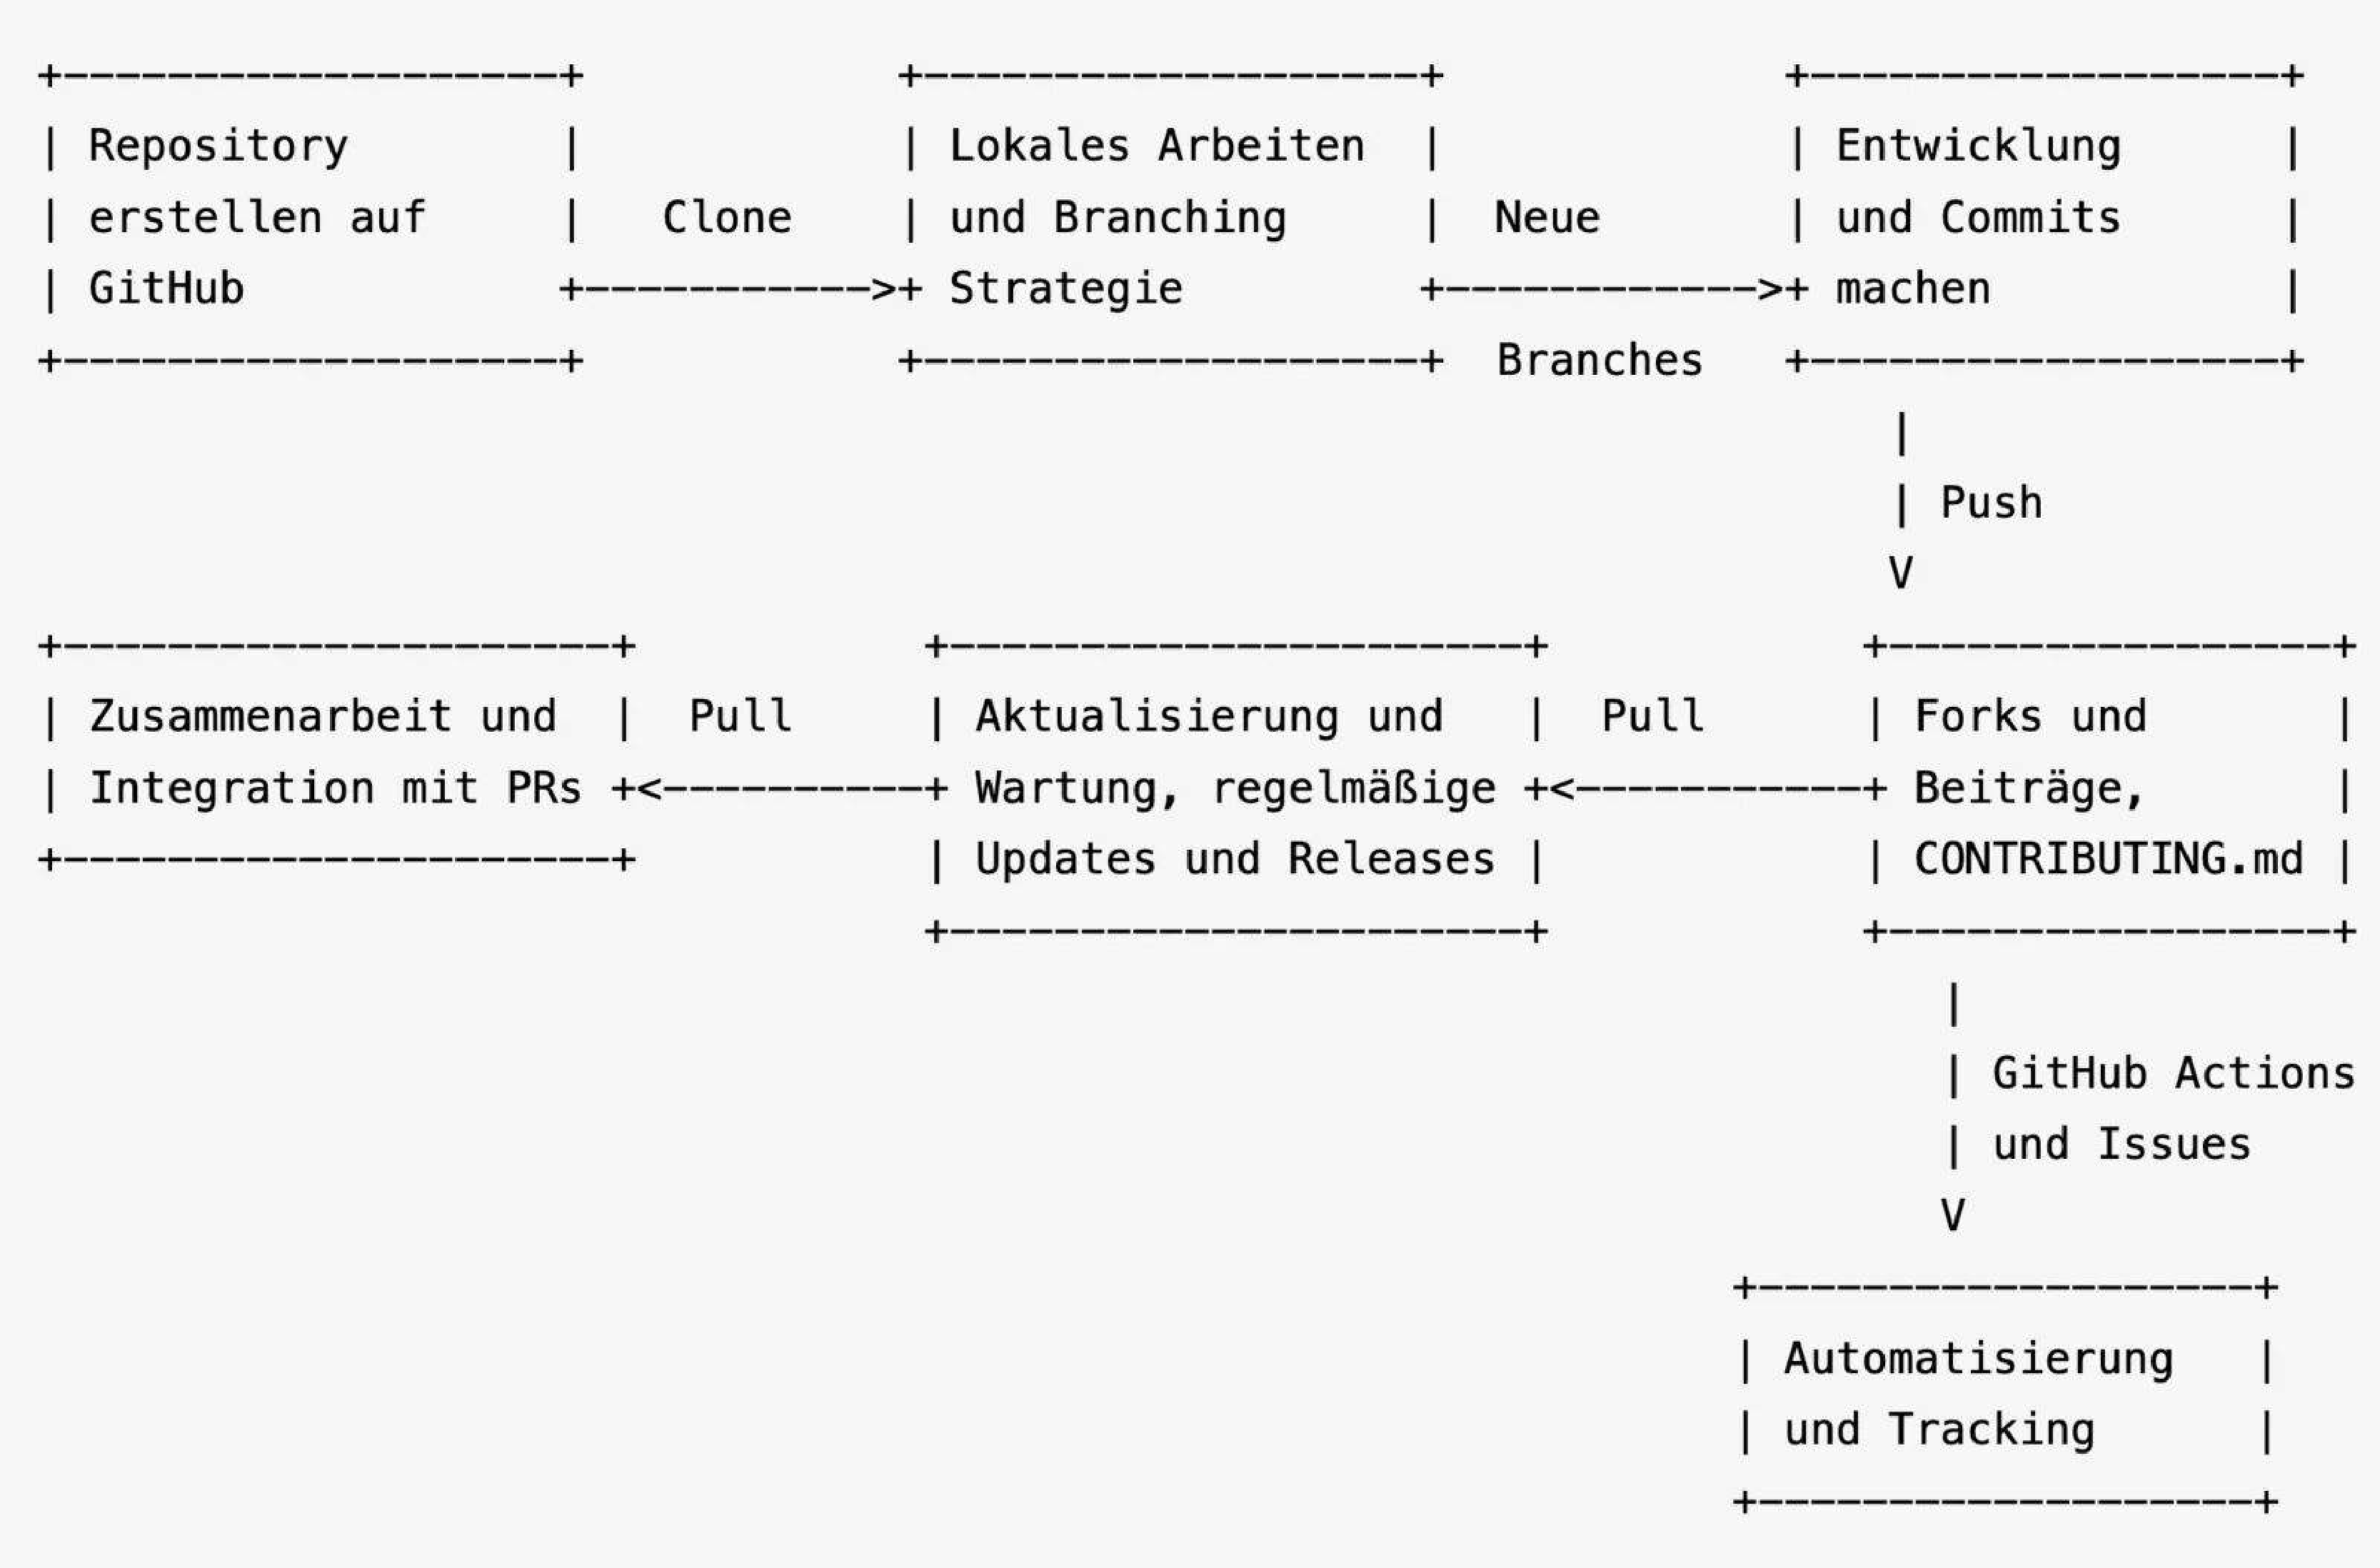
\includegraphics[width=0.8\textwidth]{images/Git-Python-Entwicklung.pdf}
%\floatnotes{}
%\label{fig:}
\caption{Git-Python-Entwicklung}
\end{figure}

%% Anhang
%\clearpage
%\appendix

\clearpage
\printbibliography
\end{document}